%% 
%% Latex template to System Architecture Document
%% Author: Dario A. Palminio
%% LaTeX version 2.0
%% OS: Ubuntu
%% Editor: LaTeXila 2.4.0
%% 

\documentclass[a4paper,11pt]{book}
\usepackage[T1]{fontenc}
\usepackage[utf8]{inputenc}
\usepackage{lmodern}
\usepackage{graphicx}

\graphicspath{ {images/} }

\title{Daro Generic Persistence v1.0 - Software Architecture}
\author{Dario A. Palminio}

\begin{document}

\maketitle
Licence: Creative Commons by-sa 4.0
\newline
https://creativecommons.org/licenses/by-sa/4.0/
\newline

Documentation control

%% Document Version Control (Table)
\begin{table}[h]
\begin{tabular}{lllll}
\cline{1-4}
\multicolumn{1}{|l|}{Date}       & \multicolumn{1}{l|}{Author}         & \multicolumn{1}{l|}{Version} & \multicolumn{1}{l|}{Detail}   &  \\ \cline{1-4}
\multicolumn{1}{|l|}{05/05/2015} & \multicolumn{1}{l|}{Dario Palminio} & \multicolumn{1}{l|}{1.0}     & \multicolumn{1}{l|}{Creation} &  \\ \cline{1-4}
                                 &                                     &                              &                               &  \\
                                 &                                     &                              &                               & 
\end{tabular}
\end{table}
%% 

\tableofcontents

\chapter{Introduction}
Generic Persistence is un component (package) that implements DAO Generic Persistence in Java.

\section{Purpose of the document}
The purpose of this document is to show the general architecture of a Java component called "Daro Generic Persistence".

\section{Audience}
Because the document is public license (Creative Commons by-sa 4.0) it was written for anyone interested audience.

\chapter{Architecture}
% text

\section{Scope and Context}
The Generic Persistence component consists of a JAR package ("com.daro.persistence.generic") named "DaroGenericPersistence-<VERSION>.jar" that can be used from other applications ("Concrete Persistence Service" or application) by extending the core classes.

\begin{figure}[h] % Diagram
  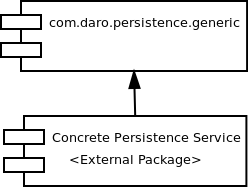
\includegraphics{generic_persistence_package_diagram}
  \caption{Context Diagram - Package Diagram}
  \centering
  \label{fig:context} %\ref{fig:context}
\end{figure}

\section{High-level Architecture}
% text

\pagebreak
\subsubsection{Class Diagram}
The classes described below belong to the package named "com.daro.persistence.generic".

\begin{figure}[h] % Diagram
  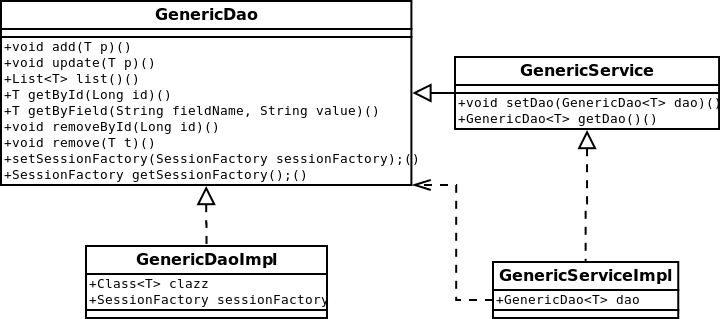
\includegraphics[width=\textwidth]{generic_persistence_class_diagram}
  \caption{General class diagram - high level}
  \centering
  \label{fig:generic_persistence_class_diagram} %\ref{fig:generic_persistence_class_diagram}
\end{figure}

\pagebreak
\subsubsection{Example of Client}
Here's a way to use the component. This example corresponds to the component testing.

\begin{figure}[h] % Diagram
  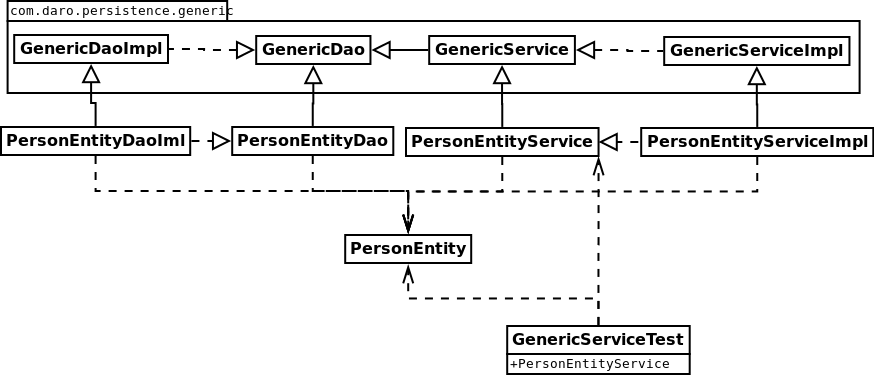
\includegraphics[width=\textwidth]{generic_persistence_class_diagram_to_use}
  \caption{Example of how to use - diagram}
  \centering
  \label{fig:generic_persistence_class_diagram_to_use} %\ref{fig:generic_persistence_class_diagram_to_use}
\end{figure}

\end{document}
